\documentclass[openany]{book}
\usepackage{tabularx}
\usepackage{graphicx}

\title{Lib2geom Manual}

\newcommand{\code}[1]{\textsf{#1}}

\begin{document}
\maketitle{}

\chapter{Overview}

\section{Introduction}

This manual focuses on the lib2geom computational geometry framework.
The main goal of this framework is the eventual replacement of
Inkscape's multiple and shoddy geometry frameworks. As with any decent
module or lib, 2geom is designed to achieve the desired functionality
while maintaining a generality encouraging usage within other
applications.  The focus on robust, accurate algorithms, as well as
utilization of newer and better representations makes the lib
very attractive for many applications.

\section{Design Considerations}
2Geom is written with a functional programming style in mind.
Generally data structures are considered immutable and rather than
assignment we use labeling.  However, C++ can become unwieldy if
this is taken to extreme and so a certain amount of pragmatism is
used in practice.  In particular, usability is not forgotten in the
mires of functional zeal.

The code relies strongly on the type system and uses some of the more
'tricky' elements of C++ to make the code more elegant and 'correct'.
Despite this, the intended use of 2Geom is a serious vector graphics
application. In such domains, performance is still used as a quality
metric, and as such we consider inefficiency to be a bug, and have
traded elegance for efficiency where it matters.

In general the data structures used in 2Geom are relatively 'flat'
and require little from the memory management.  Currently most data
structures are built on standard STL headers\cite{stl}, and new and
delete are used sparingly.  It is intended for 2Geom to be fully
compatible with Boehm garbage collector\cite{boehm} though this has
not yet been tested.

\section{Toy-Based Development}
We have managed to come up with a method of library development
that is perfect for geometry: the development of toys exemplifying
a feature while the feature is perfected.  This has somewhat subsumed
the role of tests, and provides immediate motivation/reward for work.

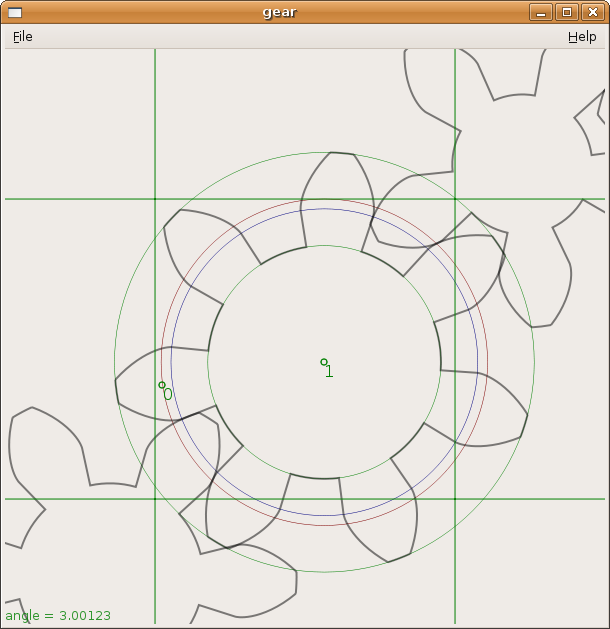
\includegraphics[width=90mm]{media/gear.png}

\chapter{Geometric Primitives}

What good is a geometry library without geometric primitives?  By this
I mean the basic stuff that every decent geometry library has:
Points/Vectors, Matrices, etc.

2geom's primitives are descendant from libNR's geometric primitives.
They have been modified quite a bit since that initial import, and
will likely change in the future.

\section{Points}

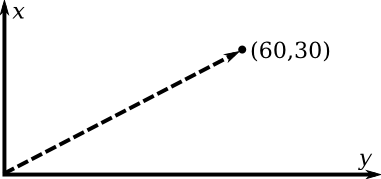
\includegraphics[height=30mm]{media/point.png}

The mathematical concepts of points and vectors are merged into the
2geom class called \code{Point}.  See Appendix A for a further
discussion of this decision.

2geom also breaks with the more traditional point \code{struct} with
\code{.x} and \code{.y} fields.  Rather, each 2geom point has a 2
element array of coordinates.

We found that the availability of \code{.x} and \code{.y} encouraged
people to attempt to inline geometry operations rather than using the
operators, perhaps in pursuit of a performance enhancement.  By using
an array, we encourage people to think about \code{Point}s as
symmetric objects and discourage direct use of the components.  We
still provide direct access for the rare occasion that it is needed.
Even in these cases, the array method prevents bugs by encouraging
iteration over the array rather than explicit element reference.

\section{Transformations}

Affine transformations are either represented with a canonical 6
element matrix, or special forms.

\subsection{Scale}

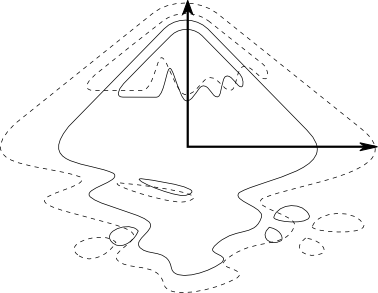
\includegraphics[height=50mm]{media/scale.png}

A \code{Scale} transformation stores x and y scaling factors.

\subsection{Rotate}

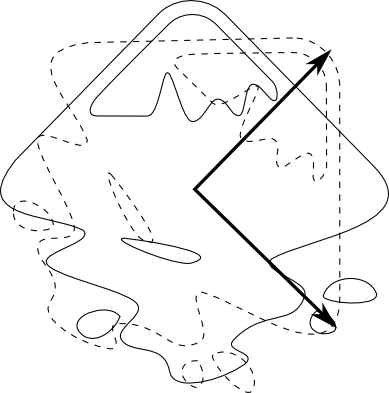
\includegraphics[height=50mm]{media/rotate.png}

A \code{Rotate} transformation uses a vector(\code{Point}) to store
a rotation about the origin.

In correspondence with mathematical convention (y increasing upwards),
0 degrees is encoded as a vector pointing along the x axis, and positive
angles indicate anticlockwise rotation.  So, for example, a vector along
the y axis would encode a 90 degree anticlockwise rotation of 90 degrees.

In the case that the computer convention of y increasing downwards,
the \verb}Rotate} transformation works essentially the same, except
that positive angles indicate clockwise rotation.

\subsection{Translate}

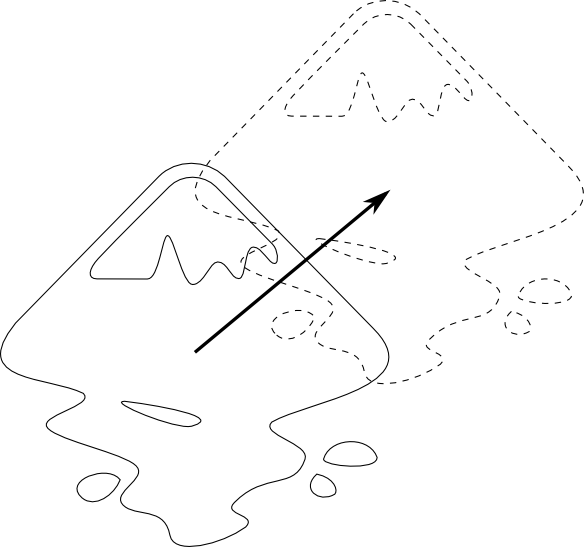
\includegraphics[height=70mm]{media/translate.png}

A \code{Translate} transformation is a simple vector(\code{Point})
which stores an offset.

\subsection{Matrix}

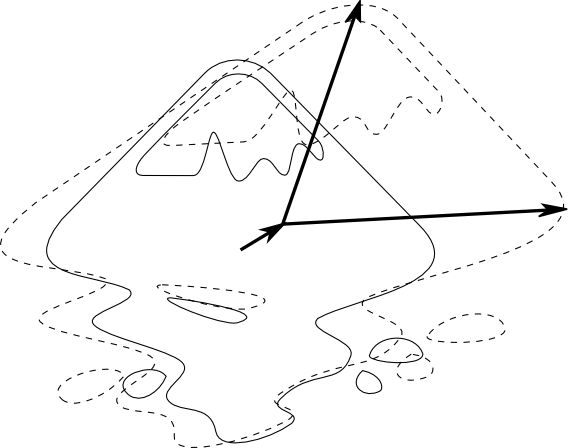
\includegraphics[height=70mm]{media/matrix.png}

A \code{Matrix} is a general affine transform.  Code is provided for
various decompositions, constructions, and manipulations.  A
\code{Matrix} is composed of 6 coordinates, essentially storing the
x axis, y axis, and offset of the transformation.  A detailed
explanation for matrices is given in Appendix B.

\subsection{D2}
The \code{D2} class takes two instances of a scalar data type and treats them like a point.  All operations which make sense on a point are defined for D2.

A \verb|D2<double>| is a \code{Point}.  A \verb|D2<Interval>| is a standard axis aligned rectangle.
\verb|D2<SBasis>| provides a 2d parametric function which maps $t$ to a point $x(t), y(t)$

\section{Bounding Structures}

2geom currently provides two classes for storing approximate bounding
regions: \code{Rect} and \code{ConvexHull}.  These are mostly intended
for use in optimization, however provide manipulations suitable for
other uses.

\subsection{Interval}

An interval is simply a pair of Coords which define a closed interval.

\subsection{Rect}

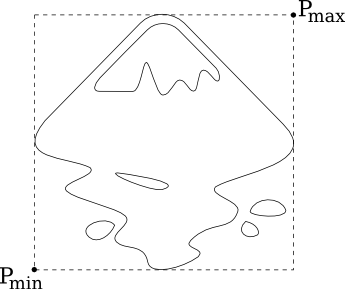
\includegraphics[height=50mm]{media/rect.png}

\code{Rect}s are rectangles with all sides parallel to the axes. 
\code{Rect}s are in fact defined as a \verb|D2<Interval>|.

\subsection{ConvexHull}

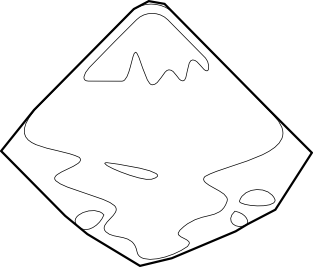
\includegraphics[height=50mm]{media/convex.png}

Currently there are two implementations:
\begin{description}
\item[convex-hull.h] is the inkscape version using rectangles.
\item[convex-cover.h] is partial implementation done with a set of points in clockwise direction.
\end{description}

\subsubsection{Operations}
\begin{description}
\item[empty:] contains no points
\item[singular:] contains exactly one point
\item[linear:] all points are on a line
\item[area:] area of the convex hull
\item[furthest:] furthest point in a direction (log time)
\item[intersect:] do two convex hulls intersect?
\item[intersection:] find the convex hull intersection
\item[merge:] find the convex hull of a set of convex hulls
\end{description}

\subsection{Piecewise}
The \code{Piecewise} class manages a sequence of elements of a type as
segments and the 'cuts' between them.  These cuts are time values which
separate the pieces.  This function representation allows for
more interesting functions, as it provides a viable output for operations
such as inversion, which may require multiple SBasis to properly invert
the original.

As for technical details, while the actual SBasis segments begin on the
first cut and end on the last, the function is defined throughout all
inputs by extending the first and last segments.  The exact switching
between segments is arbitrarily such that beginnings (t=0) have
preference over endings (t=1).  This only matters if it is discontinuous
at the location.

$$
f(t) \rightarrow \left\{ 
\begin{array}{cc}
s_1,& t <= c_2 \\
s_2,& c_2 <= t <= c_3\\
\ldots
s_n,& c_n <= t
\end{array}\right.
$$

\chapter{Paths}

A \code{Path} is an ordered set of \code{Curve}s.  Each \code{Path} is $C0$ continuous.  To make multiple contours for a region, use \code{PathVector}. 

A \code{PathVector} in Inkscape is drawn in a single fill and stroke.  

This allows us lots of flexibility with what sort of elements we can
'understand', while only taking slightly more memory than a sequence
of points in the poly line or poly bezier case. 

The Curves themselves are immutable, which means that they can be shared between Paths.

There is an implicit line segment from the initialPoint to the finalPoint which is used if the path is closed.

An empty (size() == 0) path defines a naked move to.

\section{Curves}
2Geom has a diversity of curve types and conversions between them.

Curves define a continuous segments which yields points for values of
t in the range of [0,1].  The start-point is at t=0, and the endpoint
at t=1.

We require that each \code{Curve} implements virtual functions which
allow for traversers of a path to perform generic operations.  All
curves must provide functions which give a position and gradient of a
$t \in [0,1]$, bounds functions, and conversion to s-basis.

\subsection{Bezier Curve}
We use a \code{Bezier} curve class to store lines and quadratic/cubic
beziers.  This flexibility is attained by templating on order:
\code{Bezier$<1>$} is a line segment, \code{Bezier$<2>$} is a quadratic
bezier, and \code{Bezier$<3>$} is a cubic bezier.

Bezier curves have some nice properties:
\begin{itemize}
\item Affine transforming the handles also affine transforms the values.
\item The convex hull of the handles encompasses the curve.
\end{itemize}

\subsection{SVG Elliptical Arc}
The \code{SVGEllipticalArc} curve class is implemented for support of
the SVG elliptical arc.  See the svg documentation for details on this
curve.

\subsection{S-Basis Curve}
The \code{SBasisCurve} wraps the \code{MultidimSBasis$<2>$} class
described later.

\subsection{Possible Future Curve Types}
\begin{itemize}
\item Clothoids / Raphoids
\item NURBS
\end{itemize}

\chapter{S-Power-Basis Form}

2Geom provides a very powerful algebra for modifying paths.  Although
paths are kept in an extended SVG native form where possible, many
operations require approximation.  To do this we can convert a path
into a sequence of symmetric power basis polynomials, henceforth
referred to as s-basis, perform the required operations and convert
back, approximating to a requested tolerance as required.

The precise details of the s-basis form are beyond the scope of this
manual, the interested reader should consult \cite{SanchezReyes1997,SanchezReyes2000,SanchezReyes2001,SanchezReyes2003,SanchezReyes2004}.
An elementary, functional description is given in Appendix C.

Geometrically important properties:
\begin{itemize}
\item exact representation of bezier segments
\item low condition number on bezier conversion.
\item strong convergence guarantees
\item $C^0$ continuity guarantee
\end{itemize}

The following operations are implemented and are very efficient:
\begin{itemize}
\item fast conversion from all svg elements
\item basic arithmetic --- $+$, $-$, $\times$, $\div$
\item algebraic derivative and integral
\item elementary trigonometric functions: $\sqrt{\cdot}$, $\sin(\cdot)$, $\cos(\cdot)$, $\exp(\cdot)$
\item efficient degree elevation and reduction
\item function inversion
\item exact solutions for many non trivial operations
\item root finding
\item composition
\end{itemize}

All of these operations are fast.  For example, multiplication of two
beziers by converting to s-basis form, multiplying and converting back
takes roughly the same time as performing the bezier multiplication
directly, and furthermore, subdivision and degree reduction are
straightforward in this form.

\section{Implementation}
As described in Appendix C, SBasis functions have the form $f(t) \rightarrow y$.
Just S-Basis functors (in the C++ sense) alone are not enough to perform
useful geometric operations.  There are quite a few 2geom classes to
address these needs.

\subsection{SBasis}
The \code{SBasis} class provides the most basic function form,
$f(t) \rightarrow y$.  This is useful in its own right, as well as being an
element of constructing more complicated forms.  \code{SBasis} are made
up of \code{BezOrd}s, which store from/to values for each polynomial
coefficient.

\subsection{SBasis2D}
SBasis2D provides multivariate form --- functions of the form
$f(u,v) \rightarrow z$.  These can be used for arbitrary distortion
functions (take a path $p(t) \rightarrow (u,v)$ and a pair of surfaces
$f(u,v),g(u,v)$ and compose: $q(t) = (f(p(t)), g(p(t)))$.

Subdivision for surfaces may be done with either quadtrees or kd-trees.

In general it is recommended to use the \verb|Piecewise<SBasis>| type rather than the SBasis type directly, as it manages the domain arithmetic automatically.  It also automatically subdivides when necessary to improve accuracy/convergence.

\chapter{2D databases}

2Geom provides an implementation of a 2D database using quad trees and
using a list.  Quad trees aren't the best data-structure for queries,
but they usually out perform the linear list.  We provide a
standard interface for object databases with performance guarantees
and provide a set of useful operations Operations:

\begin{description}
\item[Insert:] given a bounding box and a 'reference', insert into the db
\item[Delete:] given a bounding box and a 'reference', delete from the db
\item[Search:] given a box, find all objects that may interact with this box
\item[Cast:] given a path (including rays) return a list of objects that interact with the path, roughly sorted by path order
\item[Shape query:] given a closed path, find all objects whose bounding boxes intersect path.  (this and cast are nearly the same)
\item[Nearest:] given a point (or maybe box) find the nearest objects, perhaps as a generator to get all objects in order.  To do this, we walk around the quad tree neighbourhood, pushing all the elements into a priority queue, while the queue is empty, move out a bit.  Nearest could be manhattan, max norm or euc?
\item[Binary:] take two dbs, generate all pairs that have intersecting boxes.
\item[Sweep:] traverse the tree in say y order, maintaining a y-range of relevant objects. (to implement sweepline algorithms)
\item[Walk:] traverse the tree in an arbitrary order.
\end{description}

\chapter{Topological operations: sweepline, boolops, sanitize}
\section{Layer 1: Path Intersection}

\begin{verbatim}
src/path-intersection.cpp
src/path-intersection.h
src/crossing.h
src/crossing.h
src/toys/winding-test.cpp
\end{verbatim}

\subsection{Winding Number:}
 the number of times the path goes around a particular point. Since paths are closed, the result is always integral. A counter-clockwise rotation corresponds to a positive wind, whereas a clockwise rotation is represented as a negative wind. Here, and throughout, the terms clockwise and counter-clockwise refer to the standard mathematical coordinate system rather than the computer, inverted y-axis, coordinate system.

\subsection{Crossing:}
 a location where two paths cross. This is a subset of the intersections of the paths, with the requirement that the winding must change. Crossings are stored as two time values and a boolean indicating the relationship between the curves at the crossing. A particular time value corresponds to the point on curve i at f, where i is the integral part, and f is the fractional part. This boolean is useful for making decisions during a traversal of crossings. It is defined as the sign of the cross product of the derivatives. When the paths are regions with the same winding, this indicates that along B, A crosses 'outside'.

\subsection{Winding functions:}

\verb|int winding(Path, Point);|
\verb|bool path_direction(Path);|  —  assumes the path is simple (like a region)
\verb|bool contains(Path, Point, bool even-odd = true);|  —  convenience wrapper around winding

There are a few convenience typedefs for the popular crossing collections:
\verb|typedef std::vector<Crossing> Crossings;|
\verb|typedef std::vector<Crossings> CrossingSet;|

The intersection system is designed to be modular, so that different algorithms may be used. The current algorithms are generic, and apply to anything that implements Curve. A custom curve type might provide an algorithm with special cases, and default to the generic algorithms. The following crossing functions use the DefaultCrosser, which is currently a simple binary search.

\verb|Crossings crossings(Path, Path);|  —  finds the crossings between two paths
\verb|CrossingSet crossings(std::vector<Path>, std::vector<Path>);|  —  finds the crossings between two sets of paths.
Layer 2: Regions

\begin{verbatim}
src/region.cpp
src/region.h
\end{verbatim}

\subsection{Region:}
A limited point-set, defined by a boundary. This boundary is stored as a simple (non-self-crossing) path. Regions with positive winding (counter-clockwise) include points which are inside the boundary (fills), whereas Regions with negative winding include all points outside the boundary (holes). It also caches information such as winding direction and bounding box.

Most of the public api for region simply wraps and caches queries to a Path. It also provides various convenience functions such as \verb|as_fill| and \verb|as_hole|. Region should usually only be used by clients of this library when dealing with paths with the same invariants as regions.
\section{Layer 3: Shapes}

\begin{verbatim}
src/shape.cpp
src/shape.h
src/toys/boolops.cpp
\end{verbatim}

\subsection{Shape:}
A point-set upon which boolean operations may be performed. Shapes are defined by a list of regions, where the resulting point-set is the cumulative intersection. Though it may be figured out from the regions, shapes also store whether the most outer paths are fill or hole. In other words, it stores the value of all the points completely outside the boundary of all its constituent regions. Shapes have the following invariants:

\begin{itemize}
\item{ The regions must not cross, or intersect for more than a point.}
\item{ Filled regions only contain 'hole' regions, and vice-versa.}
\item{ The 'top level' regions are all the same type (fill or hole).}
\end{itemize}

The shape files really constitutes the main body of my work, while the other stuff is peripheral support. It contains the algorithms which perform boolean operations and sanitization on shapes.

The most important function looks like this:

\verb|Shape shape_boolean(bool, Shape, Shape, CrossingSet);|

If the initial boolean is false, the function unions the shapes. If it is true, it intersects them. The CrossingSet contains the crossings between the regions of the two shapes (an overload of this function allows omission of this parameter). The functions operation is actually surprisingly simple. It traverses the crossings, keeping track of which it has hit, collecting portions of path as it goes, until it reaches a crossing it has already visited, at which point it stores the path and starts again at an unvisited crossing.

The real magic happens in the traversal. It took me quite a long time to really figure it out, but eventually I realized that quite simple logic would allow for traversing intersecting sets of regions correctly. If the boolean input doesn't equal the direction of the crossing, path A is followed, if they are equal, the path B is followed. I actually figured this particular bit fairly early on, but it was with a pair of regions. At the time I had no idea it could also work for doing boolean operations on sets of regions.

While the previous function contains the main code, the actual public function intended for public use is quite different.
\verb|Shape boolop(Shape, Shape, unsigned)|

It takes the two shapes, and a flag integer specifying which of 16 boolean operations to perform. These flags use the first 4 bits to represent a boolean truth table. This is the function which is used in the boolops toy. Half of the operations, the complements, deal with cases where the output shape is filled in areas where neither of the input shapes are. The binary complement operation(~) applied to the flags, will yield flags specifying the complementary boolean operation. 6 of the combinations of flags don't even call \verb|shape_boolean| - the various identity, inversion, and none/all operations.

\begin{verbatim}
src/sweep.cpp
src/sweep.h
src/toys/sweep.cpp
src/tests/intersection-test.cpp
\end{verbatim}

These are some support algorithms which provide a sweep on bounds, for efficient intersections between sets of bounded objects.
\section{Current Issues}

The main current deficiency is the sanitizer. I've only recently managed to get a path uncrosser somewhat working. I have a variety of sanitization methods implemented to various degrees, yet have only recently figured out the real reasons I haven't yet gotten it fully functioning. I hope to fix it soon, so that boolops may be used as a live-path-effect within inkscape (the live-path-effects project is a Summer-of-Code project). I think this is a good way to introduce the new boolean operations, and I definitely want my work to be used.

There's also some code which is currently unused:

I have an implementation of intersection routines which splits paths into monotonic portions, and uses the properties of these sections to perform very fast intersection. It works somewhat, but there are bugs I haven't had time to work out, which make the current implementation unstable. This intersection algorithm is especially valuable for self intersections, as monotonic splits are already required.

\section{Possible Future Design Changes}

It may be possible for the boolean operations to return a set of portions. When the actual path data is required, the portion operations would be applied. The actual boolean operations would take no time to execute, as all the computational load would be in the crossing-finder and path synthesizer. This would also work for the sanitization step, saving many spurious portions. The portions found in the boolean operations could be composed onto those produced by the sanitization routine, so that the unnecessary intermediary paths between sanitization and boolean operations are never generated.

The current representation of crossings between sets of paths is fairly awkward. The main core of the data structure, storing times and the direction boolean is fine, the main issue is the storage methods of collections of these crossings. I've come to realize it's actually one of the main reasons that sanitization is as hard as it has been. I've figured out that a better representation would be for each crossing to store pointers to the next and previous crossings along both its participating paths. This would form a connectivity graph, where each vertex has a degree of 4. A dedicated structure such as this would likely be worth it, as algorithms that use it would be more efficient, simpler, and less buggy.

Without too much work, it should also be possible to do boolean operations with non-filled paths. The main change would be to have \verb|shape_boolean| handle coincident crossings, and to derive the resultant region fill from the fill of the contributing regions. This would allow all combinations of boolean operations between filled regions and paths. 

\chapter{Acknowledgements and history}

2Geom is a group project, having many authors and contributors.  The
original code was sketched out by Nathan Hurst and Peter Moulder for
the Inkscape vector graphics program to provide well typed, correct
and easy to use C++ classes.  Since then many people have refined and
debugged the code.  One of the earliest C++ification projects for
inkscape was replacing NRPoint with NR::Point.

A conspicuous absence was a Path datatype, and indeed Inkscape
developed at least 3 different internal path datatypes, plus several
others in related projects.  Considering the core importance of path
operations in vector graphics, this led to much reimplementation of
algorithms, numerous bugs, and many round trips converting between
forms.

Many attempts have been made to try and develop a single path data
structure, but all were fated to sit in random SCMs scattered across
the web.

Several unrelated projects had copied out various portions of the NR
code from Inkscape and in 2006 MenTaLguY and Nathan felt that it was
time to separate out the geometry portions of inkscape into a
separate library for general use and improvement.  The namespace was
changed from NR to Geom and a prototype for paths sketched out.
Nathan studied the state of the art for computational geometry whilst
mental focussed on the design of Paths.

Before the remerging of 2Geom with the inkscape svn HEAD it was felt
that a few smaller projects should be ported to use 2Geom.  Michael
Wybrow's libavoid advanced connector routing system was ported first.

--now.

\pagebreak

\section{People who have contributed to 2Geom}
\begin{description}
\item[Aaron C.\ Spike]
\item[Alex Mac]
\item[Fred:] livarot
\item[Javier Sanchez-Reyes]
\item[Jean-Francois Barraud]
\item[Johan B.\ C.\ Engelen]
\item[Jonathon Wright]
\item[Joshua Blocher]
\item[Kim Marriott]
\item[Marco Cecchetti]
\item[MenTaLguY]
\item[Michael J.\ Wybrow]
\item[Michael G.\ Sloan]
\item[Nathan J.\ Hurst]
\item[Peter J.\ R.\ Moulder]
\end{description}

\chapter{Appendix}
\renewcommand{\thesection}{\Alph{section}}

\section{Geometric Points}
In standard geometry, points and vectors are quite distinguished: a
point is a location, whereas a vector is an unbased direction and
magnitude.  Allowed operations on vectors and points also vary:

\begin{tabular}{r l}
  $P - P$ & $= V$ \\

  $P - P$ & $= V$ \\

  $P + V$ & $= P$ \\

  $P - V$ & $= P$ \\

  $V + V$ & $= V$ \\

  $V - V$ & $= V$ \\

  $V \times S$ & $= V$ \\

  $V \div S$ & $= V$ \\
\end{tabular}

Here, $P$ represents points, $V$ represents vectors, and $S$ scalars.

Ideally we would render these restrictions in code, as they would
reinforce algorithm correctness.  This is because as far as arithmetic
operations go, the above are all that you sanely require, unless you
are prematurely optimizing.

\section{Understanding Matrices}

\section{S-Power-Basis Explanation}

\section{Concepts}

The C++ Standard Template Library\cite{stl} introduces the notion of
\emph{concepts}\cite{stl_concepts}, which specify families of types related
by a common interface.  In template-based programming with the STL, concepts
serve a similar purpose to type classes in Haskell.  While, unlike Haskell's
language-level support for type classes, concept-checking is not directly
supported by the C++ compiler or language, C++ libraries have been written
which use template techniques to provide compile-time checking and enforcement
of concepts\cite{boost_concept_check}.

There are several important lib2geom concepts in this sense:

\subsection{ScalarFunction}

\subsubsection{Description}

Scalar functions are C++ function objects which behave like functions
with type {\tt double (double)}.  They take a single time value and return
a scalar, and are defined over at least the interval $[0, 1]$.

\subsubsection{Refinement of}

\subsubsection{Associated types}

\subsubsection{Notation}

\begin{tabular}{r l}
  {\tt X} & A type which models ScalarFunction \\
  {\tt a} & An object of type {\tt X} \\
  {\tt t} & A time value of type {\tt double} \\
  {\tt n} & A count of type {\tt unsigned int} \\
\end{tabular}

\subsubsection{Definitions}

\subsubsection{Valid expressions}

\begin{tabularx}{300pt}{X l X l}
  Name & Expression & Type requirements & Return type \\
  Evaluate & {\tt a(t)} & & {\tt double} \\
  Evaluate & {\tt a.valueAt(t)} & & {\tt double} \\
  Evaluate with derivatives & {\tt a.valueAndDerivativesAt(t, n, out)} & {\tt out} should be a model of OutputIterator whose {\tt value\_type} is convertible to & {\tt void} \\
  Range & {\tt a.fastRange()} & & {\tt Range} \\
  Range & {\tt a.exactRange()} & & {\tt Range} \\
  SBasis & {\tt a.sbasis()} & & {\tt SBasis} \\
  Subdivide & {\tt a.subdivide(start, end)} & & {\tt Piecewise<X>} \\
\end{tabularx}

\subsubsection{Expression semantics}

\begin{tabularx}{300pt}{X l l X l}
  \bf{Name} & \bf{Expression} & \bf{Precondition} & \bf{Semantics} & \bf{Postcondition} \\
  Evaluate & {\tt a(t)} & $0\le t\le 1$ & Returns the value of the function at $t$; the function must be exact at $t = 0$ and $t = 1$ and defined over the interval $0\le t\le 1$ & \\
  Evaluate & {\tt a.valueAt(t)} & $0 \le t \le 1$ & Returns the value of the function at {\tt t}; the function must be exact at $t = 0$ and $t = 1$ and defined over the interval $0 \le t \le 1$ & \\
  Evaluate with derivatives & {\tt a.valueAndDerivativesAt(t, n, out)} & $0 \le t \le 1$ & Evaluates the function and the first n derivatives at {\tt t}, writing them to {\tt out} & $n + 1$ values have been written to {\tt out} \\
  Range & {\tt a.fastRange()} & & The result should be a {\tt Range} which includes the function's range & \\
  Range & {\tt a.exactRange()} & & The result should be a {\tt Range} representing the exact range of the function & \\
  SBasis conversion & {\tt a.sbasis()} & & The result should be an sbasis approximation of the function & \\
\end{tabularx}

\subsubsection{Complexity guarantees}

\subsubsection{Invariants}

\subsubsection{Models}

\subsection{Curve}

\subsection{UVFunction}

\section{Location Sequences}

Many algorithms are more efficient on a sorted sequence of locations,
than calling the function repeatedly for each.  So we have algorithms
that take a sequence of locations, assumed in order, and perform an
action on those.  For example, cutting a path at one location is
basically linear in the number of path segments, but cutting a path in
10 locations is still about the same amount of work.  Similarly,
working out the arc length for a location is about the same amount of
work as working out the arc length for 1000 locations on that path.

Many operations are best described as returning an ordered set of
locations.  For example, we have a function that returns
intersections between two paths.  Rather than return just one
intersection, we might return all intersections, either in order along
the path, or in order of distance along other path.
% I don't understand the distinction between "order along the path" and "order
% of distance along the path".  As for the case of a path that goes back on
% itself, e.g. a path whose y coordinate is unchanging and whose x coordinate
% goes from 0 to 10 then back to 5 then to 15, I think most callers (including
% the dashes case below) want it to behave the same as if the y coordinate did
% change, i.e. want the same point reported three times if there's an
% intersection at x=7.  Whereas the case of a "stationary path" (bezier whose
% control points are all coincident) is considered to have just one point and
% zero length. -- pjrm.

Think about dashes: a dash is a fixed arclength offset.  So rather
than getting the location for a point at arc length 1, at arc length
2, 3, 4, $\ldots$, up to the length of the curve, instead we just ask for all of
these, and the algorithm can chug along the curve outputting the
answer for each.  The reason it is faster is because to work out the
location at arc length say 100, we basically need to work out the
length for many spots up to 100.

Perhaps we then want to split the curve at each of those points.  To
split a segment at a location first requires finding that segment,
then splitting it and finally constructing a new path to output a whole
new path so we can fit the two new segments in.  If we started at the
beginning, and split at the first location, then that would be $n+1$ steps: $n$
segs in the original, plus an extra one.  If we wanted to split at 100
points, it would be $n+1$ steps for the first, $n+2$ for the
second, $\ldots$, $n+100$ steps for the last, this would take a total of $100n +
100*101/2$ steps!  Whereas, if we split as we went along, it would take
just $n+100$ steps.

The downside is that I'll probably not provide a separate split
routine that takes a single point, to discourage people from making
exactly that mistake.

\end{document}
